\section{Problem-Analyse}

In diesem Abschnitt wird das Problem bei der Verwaltung von Texten in \ac{IKTM} beschrieben. Mit Hilfe von Interviews wird gezeigt, welche typischen Arbeitsabläufe in Unternehmen existieren und welche Probleme dabei auftreten.

\subsection{Definition}

Produkt (Medium): Ein \acl{IKTM} ist ein physischer oder elektronischer Informationsträger, wie z.B. eine Broschüre oder ein Programm.

Text (Textbaustein): Damit sind die kleinsten sinnvoll identifizierbaren Bestandteile gemeint, aus denen sich der Text eines Produktes zusammensetzt. Dies sind in der Regel einzelne Sätze bei Druckmedien, können aber auch einzelne Worte sein, wie z.B. die Beschriftung einer Schaltfläche in einer Software.



\subsection{Die besondere Rolle von Text}

Fast jedes Multimedia-Produkt enthält Text, denn Text ist im Gegensatz zu Grafiken, Fotos oder Animationen ein eindeutiger Informationsträger und unterliegt viel weniger stark einer Intepretation durch den Rezipienten eines Mediums als die symbolisierte oder stilisierte Darstellung von Informationen in audiovisuellen Medien. Auch aus rechtlichen Aspekten ist Text aus den genannten Gründen der einzige verbindliche Informationsträger – bestes Beispiel hierfür ist das sogenannte „Kleingedruckte“, dass sich gerade bei inhaltlich sehr stark komprimierten Werbeformen, wie z.B. Plakat- oder Fernsehwerbung, findet.

Ist die Textmenge, die im Absatzmarketing zum Einsatz kommt, noch überschaubar, gibt es doch \ac{IKTM}, deren Hauptbestandteil Text ist. Hierunter fallen klassische Druckerzeugnisse wie Broschüren und Kataloge oder Produkte der Unternehmenskommunikation wie Jahresberichte und Pressemeldungen. Doch besonders digitale \ac{IKTM} werden oft mit großen Textmengen versehen – von der einfachen Produkt-Microsite, über Werbmittel wie Newsletter bis zur Unternehmenswebsite – die Möglichkeit Inhalte hierarchisch zu struktuieren und sogar über eine Suche zugänglich zu machen hebt eine Limitierung des Umfanges, wie bei Druckprodukten, praktisch auf.

\subsection{Erstellung von Texten in Projekten}

Alle genannten Produkte haben gemeinsam, dass ihre Erstellung in der Regel die Zusammenarbeit vieler Personen erforderlich macht. Beobachtet man den Prozess, kann man feststellen, dass es sechs verschiedene Rollen rund um die Texterstellung gibt, die ein Mitarbeiter einnehmen kann; zum Teil übernimmt eine Person dabei auch die Aufgaben mehrerer Rollen:

\begin{enumerate}
\item{Der \textbf{Informationsarchitekt} (oder Konzepter) legt die Struktur eines Produktes fest und damit auch die Art und Menge des benötigten Textes,}
\item{der \textbf{Texter} verfasst die Texte,}
\item{der \textbf{Übersetzer} überträgt die Texte in weitere Sprachen,}
\item{der \textbf{Qualitätsmanager} überwacht die Ergebnisse der Prozesse,}
\item{der \textbf{Produktbesitzer} (oder Kunde) ist für die fachlichen und rechtliche Aspekte, sowie das Festlegen der zeitlichen Rahmenbedingungen verantwortlich,}
\item{der \textbf{Produzent} ist für die Erstellung des eigentlichen Produktes verantwortlich.}
\end{enumerate}

Alle Rollen haben im Verlauf eines Projekts, zu unterschiedlichen Zeiten und mit unterschiedlichem Gewicht, Einfluss auf die Gestaltung der Texte. Es existieren auch Abhängigkeiten zwischen den Rollen, so kann ein Übersetzer erst arbeiten, wenn der Text vorliegt und vom Produktbesitzer abgenommen wurde; wird aber zu einem späteren Zeitpunkt der Text geändert, muss auch wieder der Übersetzer neu beginnen.

\begin{figure}[htb]
\begin{center}
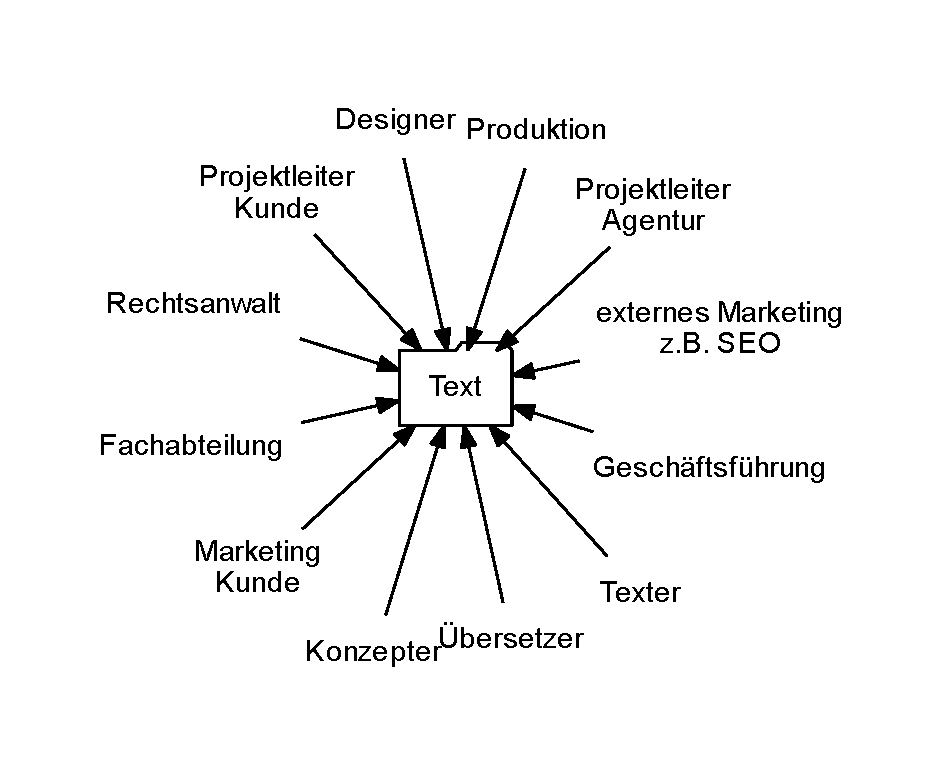
\includegraphics[width=\textwidth]{media/chart-2.pdf}
\end{center}
\caption{Bei der Erstellung von Texten für \ac{IKTM} beteiligte Personen}
\label{chart:2}
\end{figure}

Neben den menschlichen Einflüssen gibt es auch projektbedingte Einflüsse auf Text. Zum einen gibt es Situationen in denen in Texten bestimmte Informationen enthalten sind, die einen zeitlichen Aspekt abbilden. Ein Bespiel sind Gewinnspiele: Verschieben sich durch Probleme während dem Projekt die Zeiten, ab wann ein Produkt beim Rezipienten vorliegt, müssen auch evtl. knapp kalkulierte Gewinnspieltermine angepasst werden. Des weiteren gibt es oft erst gegen Ende eines Projektes Textänderungen aus der Rechtsabteilung des Kunden, da aus zeitlichen und finanziellen Gründen Anwälte gerne erst dann konsultiert werden, wenn Projekte kurz vor der Fertigstellung stehen. Da es Kunden von den Office-Produkten her gewöhnt sind, mit Text umzugehen, und sie aus eigener Erfahrung vermeintlich wissen dass Texte schnell geändert sind, erwarten sie auch, dass die Texte im Produkt bis zum Schluss geändert werden können.

\subsection{Textspezifische Aufgaben}

\begin{figure}[htb]
\begin{center}
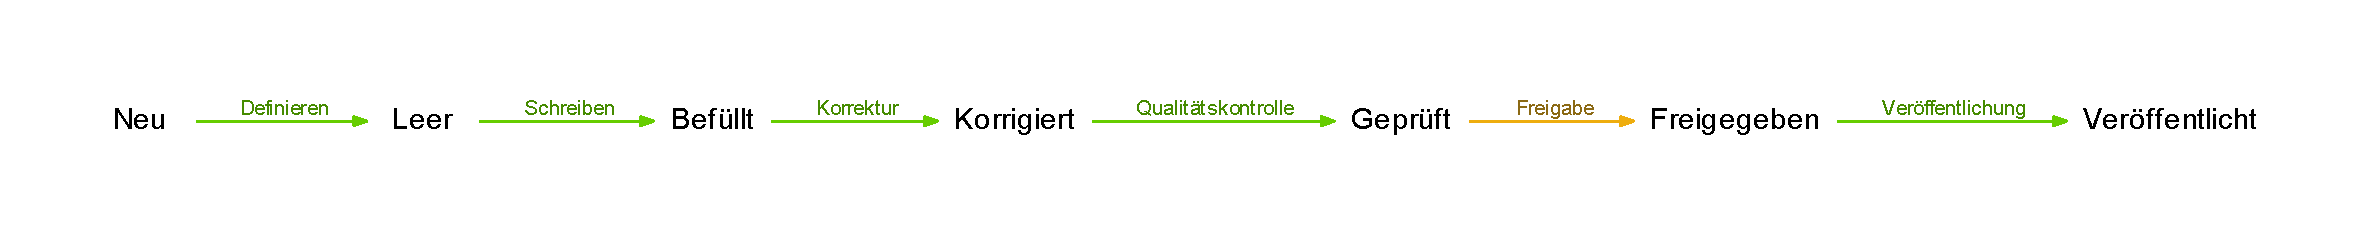
\includegraphics[width=\textwidth]{media/chart-3.pdf}
\end{center}
\caption{Operationen bei der Erstellung von Texten}
\label{chart:3}
\end{figure}

Betrachtet man die Arbeiten in Zusammenhang mit Text lassen sich diese in 6 eigenständige Operationen unterteilen:

\begin{enumerate}
\item{Durch \textbf{Definieren eines Textbausteines} wird festgelegt, wie der benötigte Text beschaffen sein muss. Die Aussage „Wir brauchen an dieser Stelle eine Überschrift“ ist ein Beispiel für diese Operation. Sie legt fest, wie der Textbausteine gestaltet werden muss, um die ihm zugedachte Aufgabe zu erfüllen. Neben der Angabe zur Platzierung auf dem Medium durch „an dieser Stelle“ wird implizit durch „eine Überschrift“ eine Angabe zur inhaltlichen und visuellen Gestaltung getroffen; Überschriften sollen kurz und knapp sein und ihre visuelle Gestaltung wird durch den Styleguide des Projektes festgelegt.}
\item{Das \textbf{Schreiben eines Textes} befüllt einen Textbaustein mit einem Text in einer Sprache. Bei diesem Vorgang wird der Text entsprechend der Vorgabe aus der Beschreibung als Original erstellt oder aus Quellen außerhalb des Projektes kopiert und eingefügt. }
\item{In der \textbf{Korrektur} wird der Text inhaltlich und grammatikalisch überprüft und entsprechend angepasst. Der Korrektor muss dabei für eine grammatikalische Überprüfung des Textes kein Fachwissen bezogen auf das Projekt haben. Ist diese Fachwissen vorhanden, kann eine inhaltliche Korrektur vorgenommen werden.}
\item{In der \textbf{Qualitätskontrolle} wird der Text dahingehend überprüft, ob er den Anforderungen gemäß der Beschreibung und inhaltlichen Vorgaben, auch hinsichtlich des gesamten Projektes entspricht. }
\item{Durch die \textbf{Freigabe} wird der Text abgenommen und kann nun in das Endprodukt übernommen werden.}
\item{Durch die \textbf{Veröffentlichung} wird der Text in das Endprodukt eingebracht.}
\end{enumerate}

\begin{figure}[htb]
\begin{center}
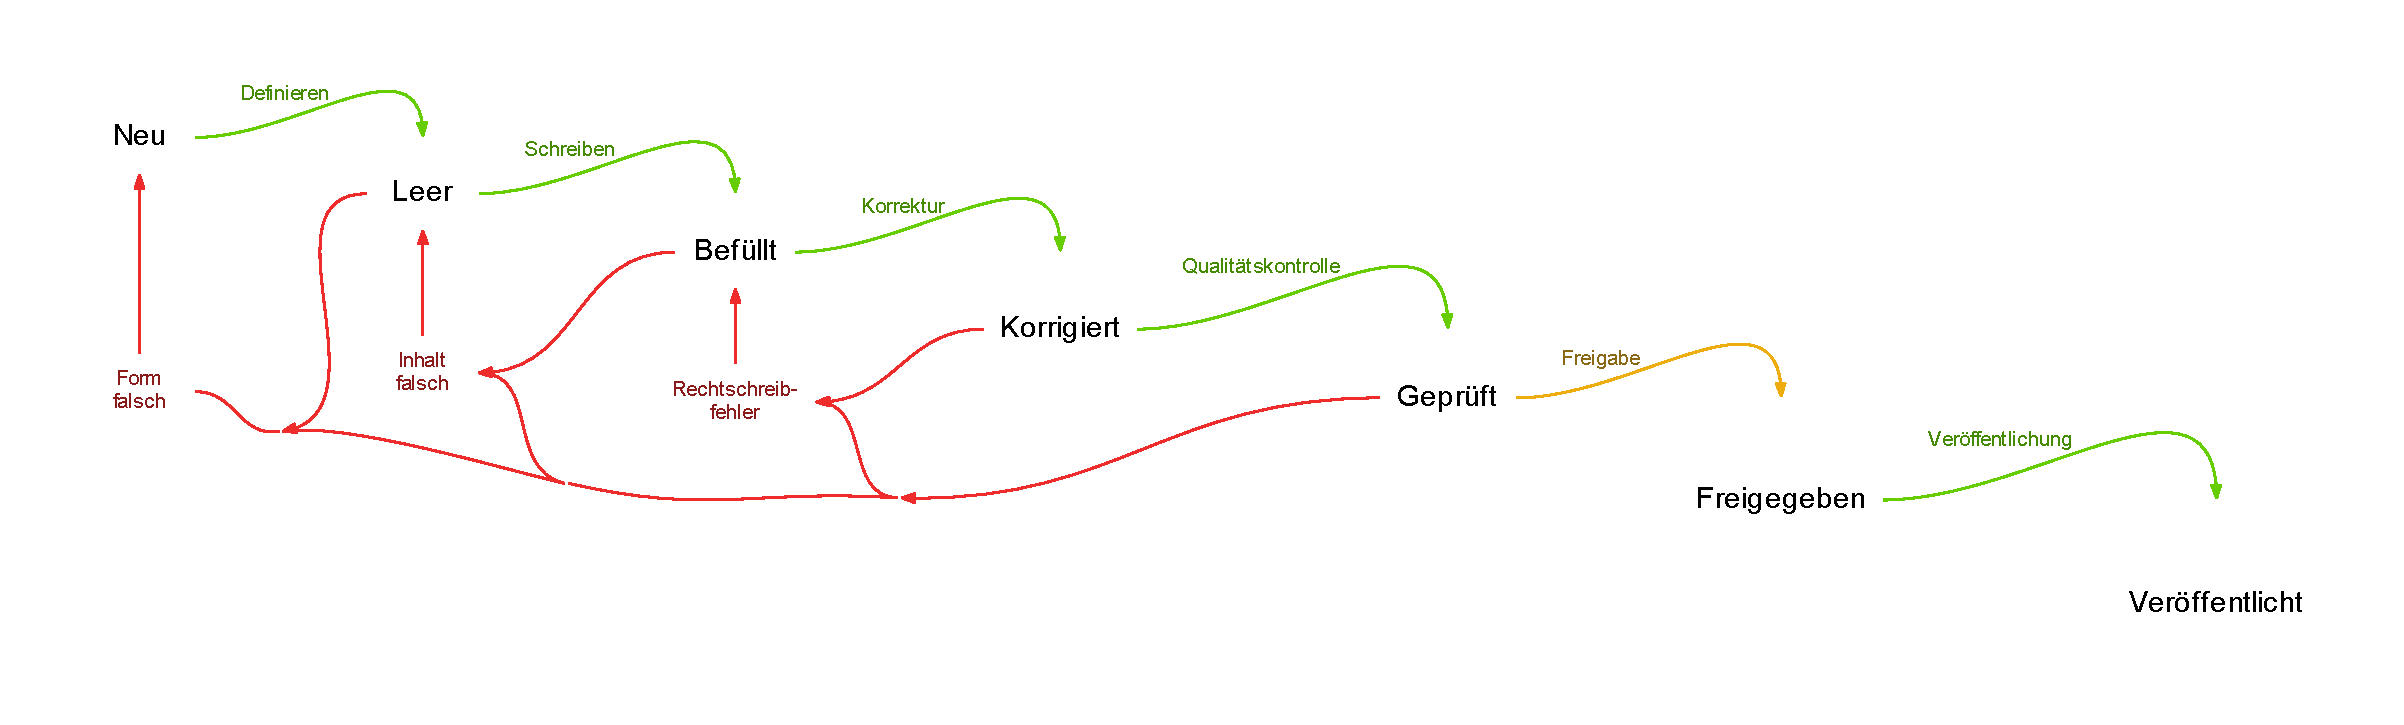
\includegraphics[width=\textwidth]{media/chart-4.pdf}
\end{center}
\caption{Operationen bei der Erstellung von Texten mit Qualitätskontrolle}
\label{chart:4}
\end{figure}

Diese Operationen werden auch 1:1 auf die übersetzte Version eines Textes angewendet.

\begin{figure}[htb]
\begin{center}
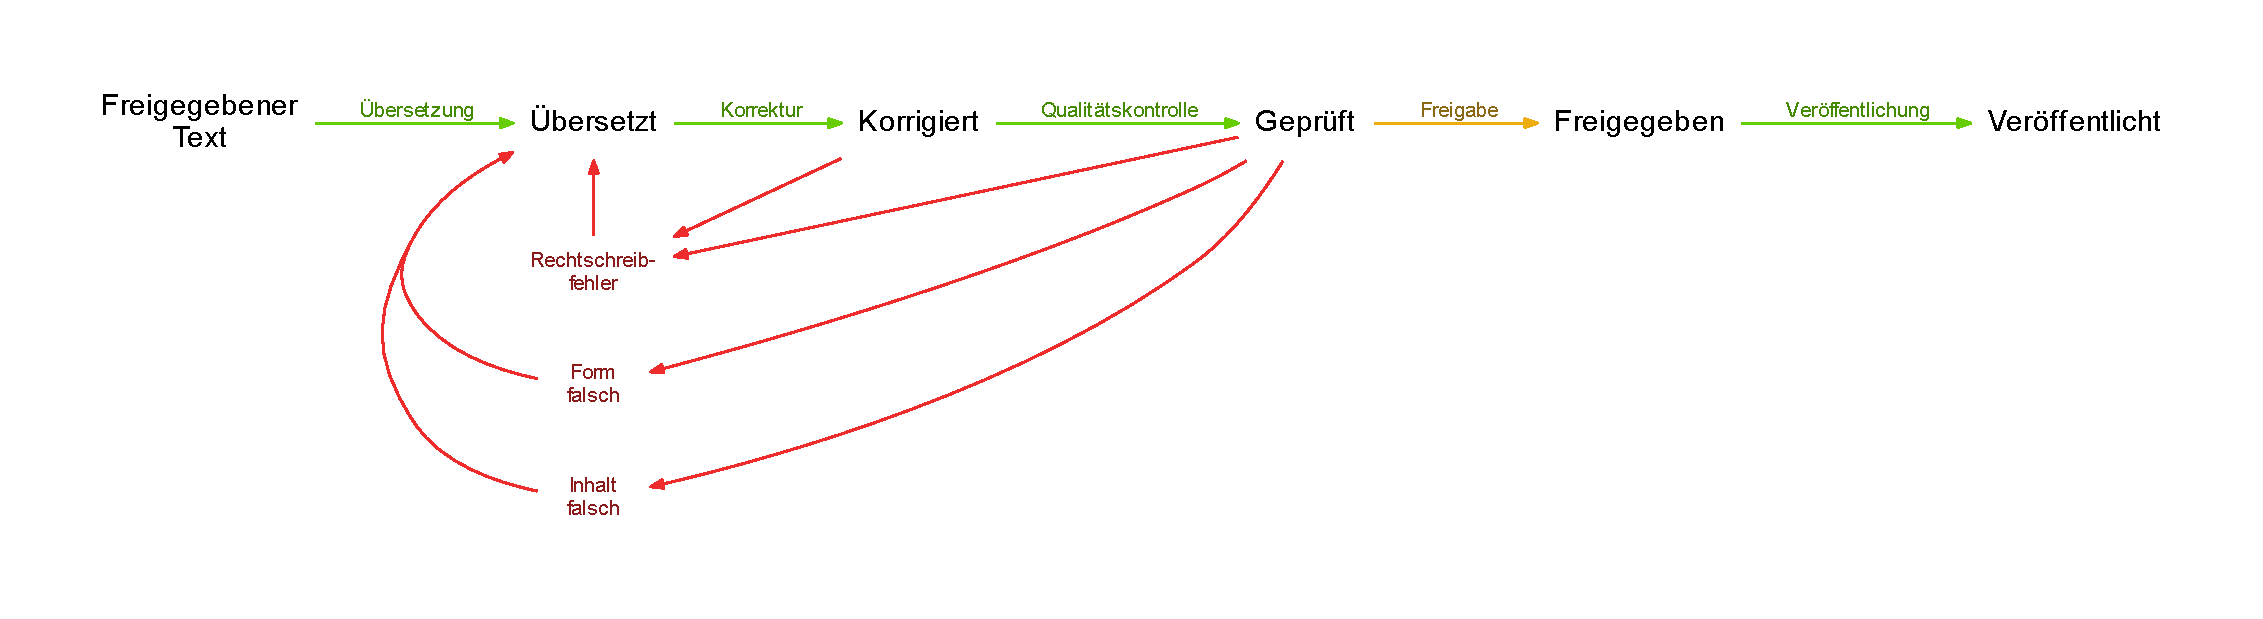
\includegraphics[width=\textwidth]{media/chart-5.pdf}
\end{center}
\caption{Operationen bei der Übersetzung von Texten mit Qualitätskontrolle}
\label{chart:5}
\end{figure}

\subsection{Microsoft Office als Standard}

\subsection{Word und Excel sind „leichtgewichtige“ Werkzeuge}

So komplex auch die Abläufe bei der Erstellung von Texten für \ac{IKTM} sind, um so erstaunlicher ist die Tatsache, dass das Werkzeug der Wahl zur Abbildung dieser Prozesse in den allermeisten Fällen \emph{Microsoft Word} oder \emph{Excel} ist. Auf den ersten Blick bilden diese Werkzeuge viele der benötigten Funktionen rund um die Textprozesse ab, aber im alltäglichen Gebrauch treten viele Probleme gerade im Bereich des gemeinsamen Bearbeitens, paralleler oder nachträglicher Änderungen und der Übertragung der fertigen Texte in den Produktionsprozess auf. Der Grund für die Wahl der \emph{Office}-Produkte liegt auf der Hand: sind sie doch in den allermeisten Unternehmen der Standard zur Textverarbeitung und sogar plattformunabhängig verfügbar – zumindest existiert die Möglichkeit das Microsoft Office-Dateiformat auf allen Platformen zu bearbeiten. Da bei allen Projektbeteiligten eine Installation von \emph{Microsoft Office} vorausgesetzt werden kann, werden sie zu „leichtgewichtige“ Werkzeugen, die vom Anwender keine zusätzlichen Aufwände z.B. bei der Installation oder Eingewöhnung erfordern. Selbst auf Plattformen, die von \emph{Microsoft Office} nicht offiziell unterstützt werden (z.B. Linux) existieren Programme mit denen das Office-Dokumenten-Format geöffnet und bearbeitet werden kann.

\subsection{Die verwendeten Office-Funktionen}

Als klassisches Textverarbeitungsprogramm verfügen Office-Programme über viele Funktionen, die die Erstellung von Texten erleichtern.

\begin{itemize}
\item{Rechtschreibkorrektur für alle üblichen Sprachen}
\item{Kommentarfunktion}
\item{Änderungsfunktionen (Nachverfolgen, wer was geändert hat)}
\item{Möglichkeit zur hierarchischen Strukturierung der Texte in Seiten, Kapitel und Abschnitte}
\item{Möglichkeit zum Anlegen eines Inhaltsverzeichnisses (in Word)}
\item{die tabellarische Ansicht in Excel ermöglicht eine übersichtliche Darstellung, meist mit der Originalsprache in der ganz linken Spalte, pro Zeile ein Text, die Übersetzungen dann in den weiteren Spalten}
\item{Export-Funktion nach PDF}
\item{Globales Suchen und Ersetzen}
\item{Formatierungsfunktionen (fett, kursiv, farblich) zum Hervorheben von wichtigen Passagen oder Markieren von Todos, etc.}
\item{Setzen von Hyperlinks (für Web-Projekte)}
\end{itemize}

Office-Dateien sind einfach auszutauschen – in Unternehmen werden die Dateien in der Regel auf einem Netzwerk-Laufwerk gespeichert. Zum Bearbeiten legt man sich eine lokale Kopie an und arbeitet in dieser Datei. Anschließend kopiert man die neue Version, meist unter Einhaltung eines bestimmten Benamungsschemas, wieder auf dem Netzlaufwerk ab. Hier können Konflikte auftreten (wenn zwei Personen gleichzeitig an der selben Datei arbeiten), diese müssen dann manuell gelöst werden. Wird die Datei direkt vom Netzlaufwerk geöffnet wird diese gesperrt und kann nur von einer Person bearbeitet werden.

Aufgrund der scheinbaren Vorteile der Office-Suite wird diese zu Beginn eines Projektes als geeignet angesehen und als Werkzeug für die Erfassung, Definition und Übersetzung der Texte eines Projektes ausgewählt.

Die im Verlauf des Projekts auftauchenden Probleme werden dann als gegeben akzeptiert, da man „nun“ damit zurecht kommen muss, um den Verlauf des Projektes nicht zu verzögern. Bei neuen Projekten wird aber die gleiche Entscheidung wieder getroffen.

\subsection{Office-Programme sind die falschen Werkzeuge}

Der Grund, warum Office-Programme wie \emph{Word} und \emph{Excel} verwendet werden ist der, dass keine keine dedizierten Lösungen existieren, die explizit die genannten Abläufe in der Textverarbeitung abbildet. Es existieren vielen Produkte aus dem Bereich der Projektverwaltungswerkzeuge, Mediendatenbanken oder Content-Management-Systemen die die Prozesse rund um die Erstellung von \ac{IKTM} vereinfachen, aber keine kann die genannten Probleme und Abläufe zufriedenstellend abbilden.

\subsection{Beispiele aus der Praxis}

Die Analyse des Problems basiert auf Interviews mit Menschen, die in ihrem Arbeitsalltag regelmäßig mit Texten zu tun haben. In diesen Interviews wurden die Personen nach ihren Erfahrungen in der Projektarbeit bezüglich Texten befragt und gebeten die aus ihrer Sicht am häufigsten auftretenden Probleme zu nennen.

\subsubsection{MAN Truck \& Bus AG: Texte für mobile Vertriebssoftware}

Markus Rüb ist als Projektleiter bei der MAN Truck \& Bus AG mit der Einführung von Tablet PCs als Vertriebshilfsmittel betraut.

\subsection{Schlussfolgerung}

